\section{Korisnički profil}

Svaki registrirani korisnik unutar aplikacije ima svoj profil koji služi kao centralno mjesto za pregled svih njegovih penjačkih aktivnosti i analizu napretka. Pristupom profilu korisniku se prikazuje sažetak njegovih penjačkih aktivnosti poput ukupnog broja posjećenih penjačkih lokacija, ukupan broj zabilježenih uspona te broj dodanih fotografija.

\begin{figure}[H]
    \centering
    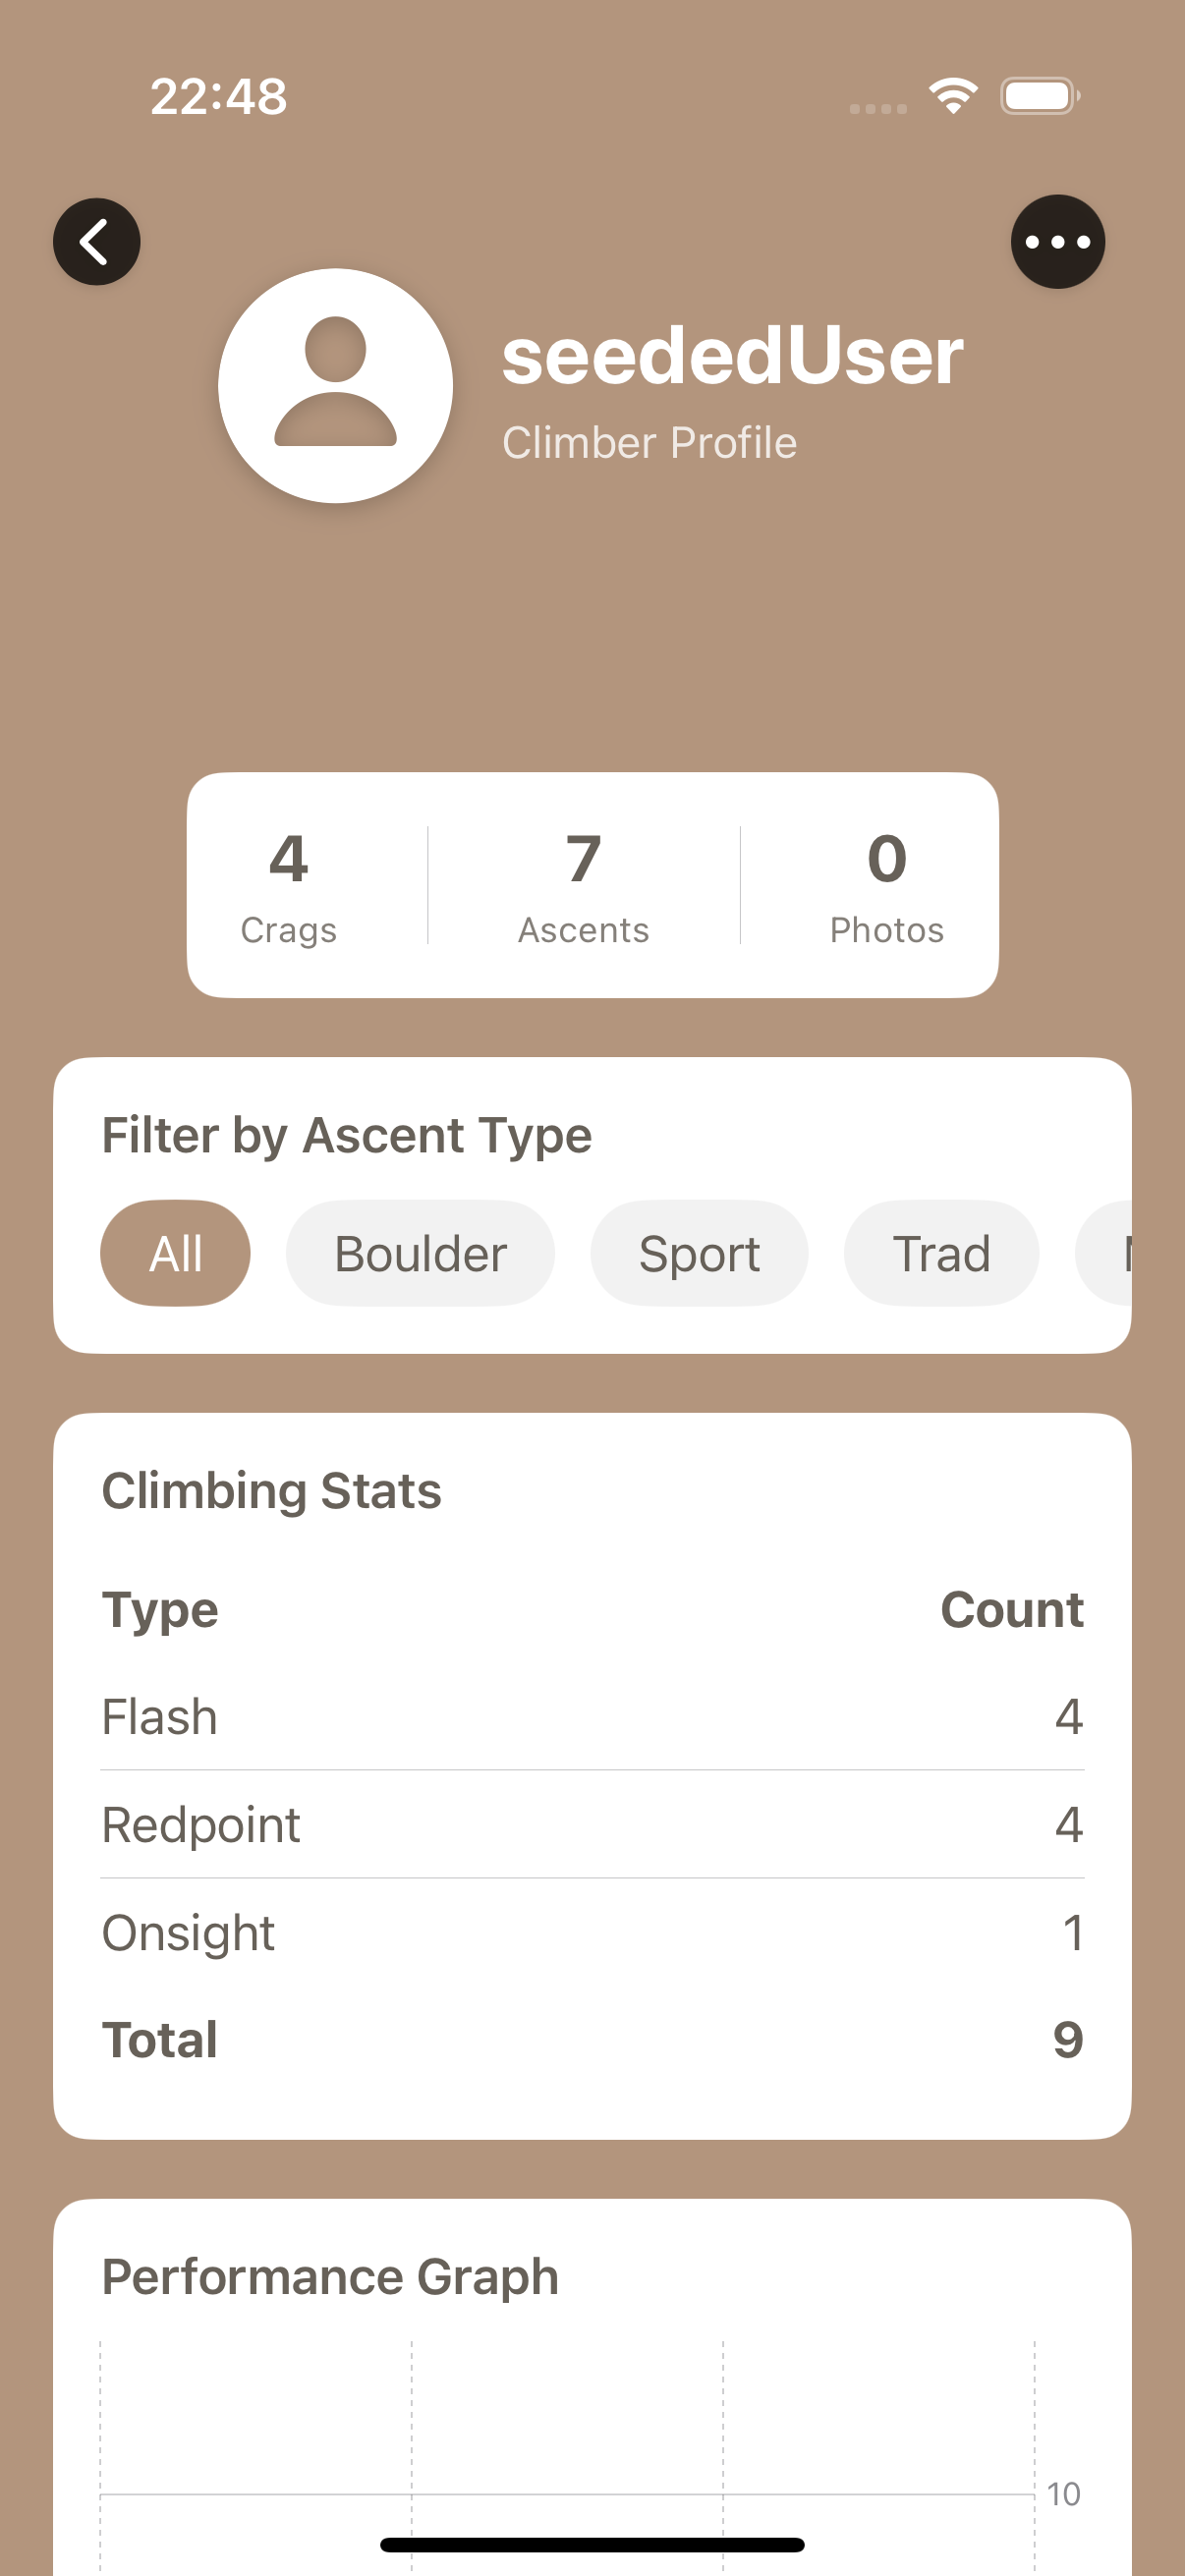
\includegraphics[width=0.35\textwidth]{images/implementacija/user_profile_1.png}
    \caption{Korisnički profil}
    \label{fig:korisnički_profil}
\end{figure}

Središnji dio profila posvećen je detaljnoj statističkoj analizi. Korisnik može filtrirati svoje uspone prema penjačkoj disciplini, poput boulder, sportsko penjanje ili tradicionalno penjanje, kako bi dobio precizniji uvid u svoje aktivnosti. Aplikacija pruža tablični prikaz broja uspona po stilu (Flash, Redpoint, Onsight), omogućujući korisniku da lako vidi koje stilove najčešće prakticira.

Za bolju vizualizaciju, podaci su prikazani i kroz dva ključna grafa. Graf performansi prikazuje distribuciju uspona po stilu, dok graf distribucije po ocjenama prikazuje barchart-om, odnosno koliko je penjačkih smjerova koje ocjene korisnik uspješno popeo. Ovi grafički prikazi omogućuju procjenu vlastitih sposobnosti i napretka kroz vrijeme. Finalno na dnu profila nalazi se i lista svih slika kojima korisnik želi istaknuti svoj profil.

\begin{figure}[H]
    \centering
    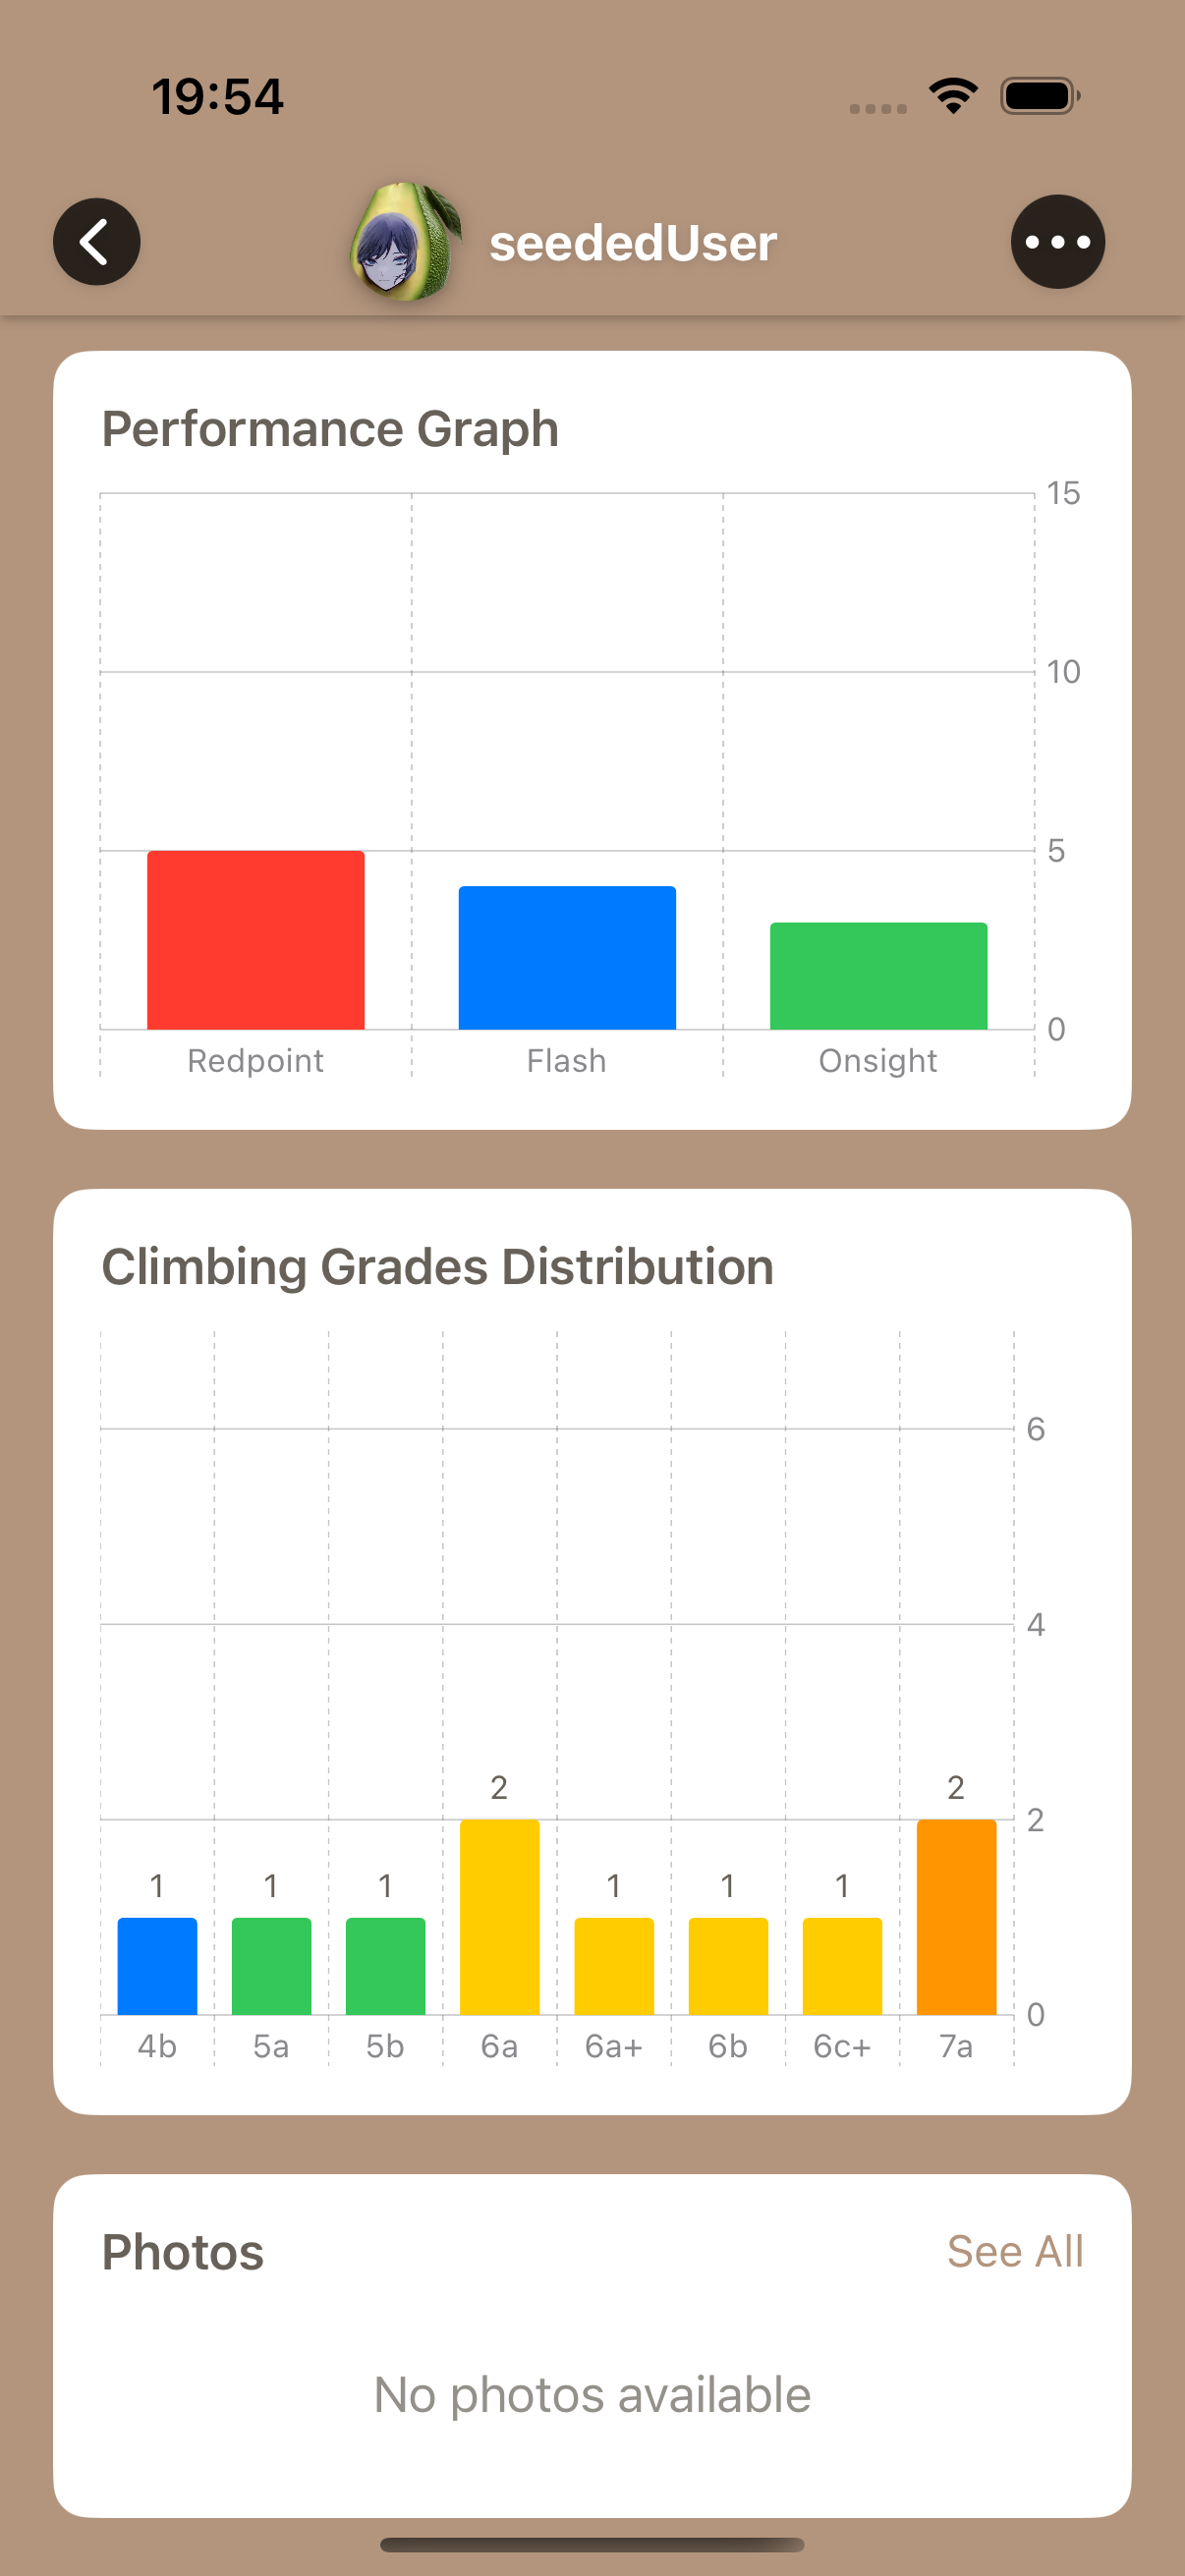
\includegraphics[width=0.35\textwidth]{images/implementacija/user_profile_2.png}
    \caption{Grafovi performansi i distribucije po ocjenama}
    \label{fig:korisnički_profil_2}
\end{figure}

Osim statistike, profil sadrži i povijest svih uspona, kronološki poredanih od najnovijeg prema najstarijem. Svaki unos u povijest sadrži sve relevantne informacije poput datuma, naziva penjačkog smjera, lokaciju, težinu, stil uspona, osobni komentar i ocjenu smjera te direktnu poveznicu na detaljni pregled samog penjačkog smjera. Ovaj dnevnik služi kao vrijedan alat za prisjećanje na prethodna penjačka iskustva.

\begin{figure}[H]
    \centering
    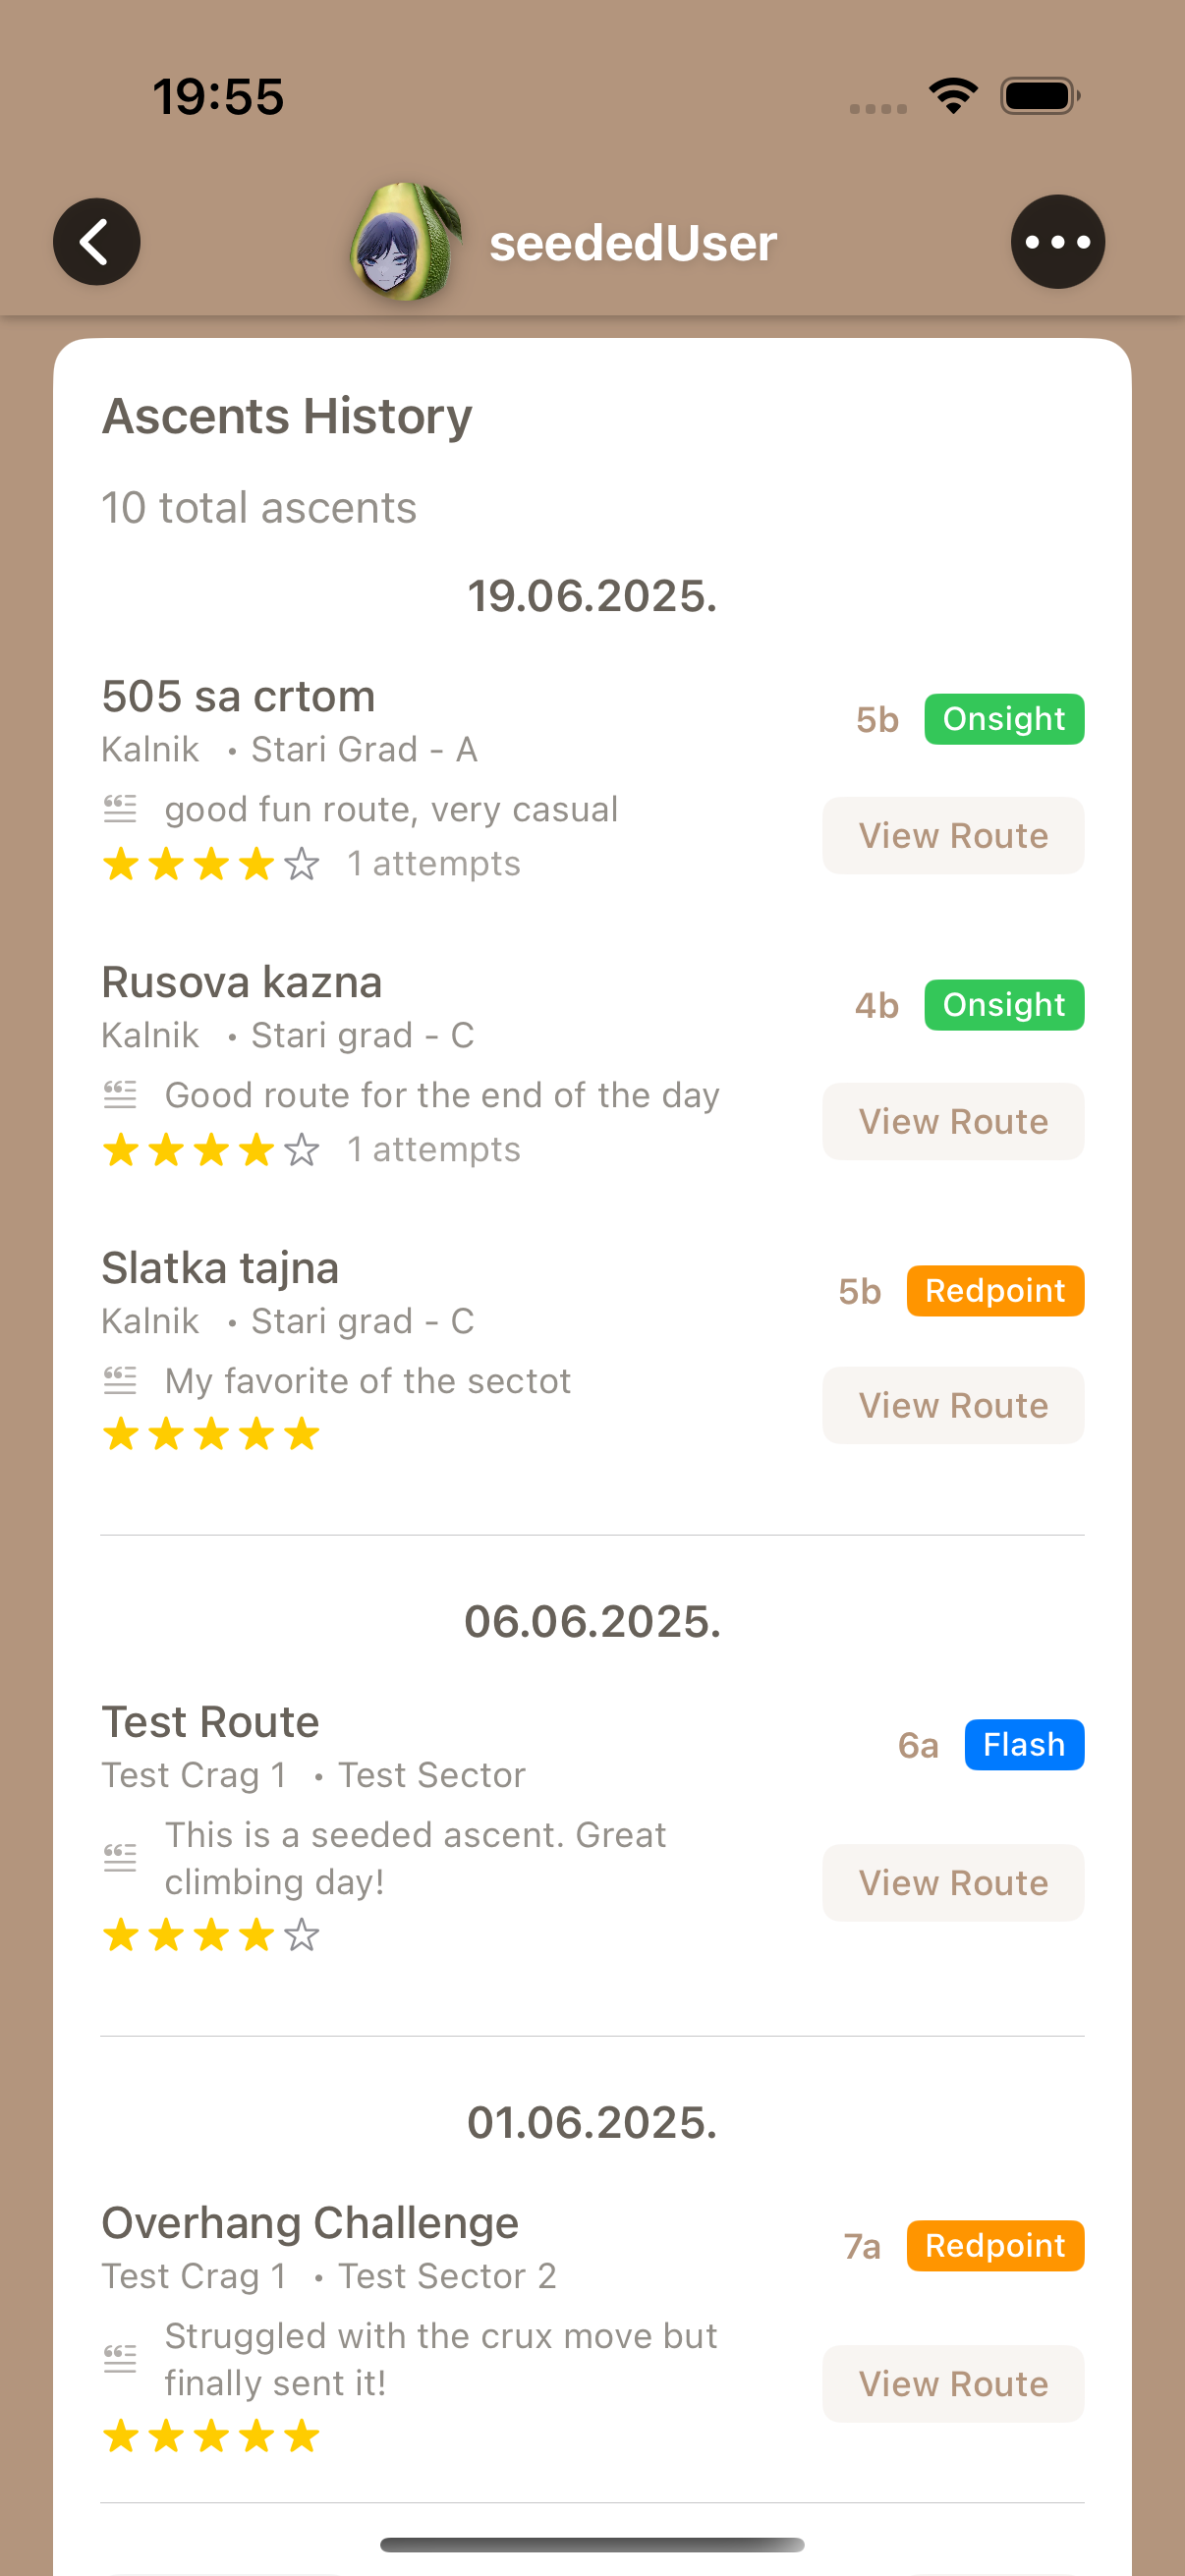
\includegraphics[width=0.35\textwidth]{images/implementacija/user_profile_3.png}
    \caption{Povijest uspona}
    \label{fig:korisnički_profil_3}
\end{figure}



Sustav "Alpinity" omogućuje dodavanje korisničko kreiranih podataka, ali na kontrolirani način kako bi se osigurala kvaliteta i točnost podataka. 

Posljednja opcija unutar izbornika je "Odjava" (eng. \textit{Logout}). Odabirom ove opcije, korisnička sesija se prekida i aplikacija se vraća na početni zaslon za prijavu.